% ----------------------------------------------------------
% Trabalhos Relacionados
% ----------------------------------------------------------
\chapter[Trabalhos Relacionados]{Trabalhos Relacionados}\label{chap:relacionados}

Nesta seção serão apresentados projetos relacionados ao tema do presente trabalho. 
Por ser um tema que agrupa dois assuntos, videoconferência e sistema de atendimento ao consumidor, e pela falta de softwares semelhantes, os dois assuntos serão analisados separadamente.

\section{Protocolos para transmissão de vídeo}

\subsection{Protocolo RTMP}

O Protocolo RTMP (\textit{Real-time Messaging Protocol}), desenvolvido pela Macromedia inicialmente como um produto proprietário e de código fechado, foi disponibilizado quando a Adobe adquiriu a empresa e liberou parte da especificação do protocolo

De acordo com sua especificação (\cite{rtpmspec}), o RMTP fornece um serviço bi-direcional de mensagens, tendo como função o \textit{streaming} de áudio, vídeo e dados de alta performance através da Internet. 

O protocolo funciona em cima de serviços de entrega de pacotes confiáveis como TCP, podendo assim ser utilizado sobre HTTP e HTTPS.

Conforme ilustrado na \autoref{fig:overview_rtmp_flash}, o RMTP é responsável por realizar a conexão entre um reprodutor Flash e um servidor de mídia Flash. 

\begin{figure}[ht!]
	\centering
		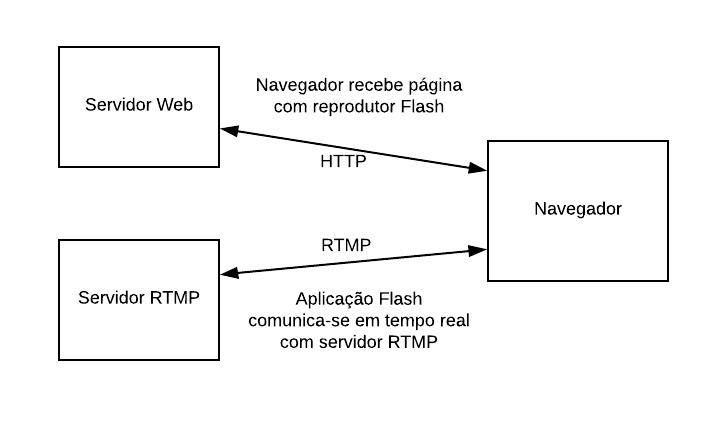
\includegraphics[scale=1]{figures/overview-rtmp-flash.png} 
	\caption{Conexão entre reprodutor e servidor Flash através do RTMP}
	\label{fig:overview_rtmp_flash}
\end{figure}

O reprodutor Flash foi inicialmente desenvolvido para reprodução de animações vetoriais bidimensionais pela Macromedia, mas acabou por tornar-se uma boa escolha para \textit{streaming} de mídia na Internet por sua capacidade de minimizar o tamanho do arquivo, economizando banda e diminuindo a latência.

Somente na versão Flash 10 o suporte a conexões P2P com RTMP foi disponibilizado. 

Há cerca de uma década, o uso do RTMP era uma escolha mais segura no lugar do \textit{WebRTC}, devido ao amplo suporte existente, resultante da presença de \textit{plugins} Flash nos navegadores, além de reprodutores nativos. No entanto, esta situação mudou completamente nos últimos anos. Alguns pontos foram decisivos para a queda do Flash e do RTMP e a ascensão do \textit{WebRTC}:

\begin{itemize}
	\item O código fechado e proprietário do RTMP não agradava certas empresas. Adiciona-se a isso o fato de elas não poderem utilizá-lo sem um reprodutor Flash.
    \item \textit{Plugins} de reprodutores Flash traziam problemas aos navegadores. Os fabricantes de \textit{browsers} começaram a notar diversos gargalos de performance e segurança. Devido à obrigatoriedade do seu uso, surgiram novas frentes para criar tecnologias de \textit{streaming}.
\end{itemize}

Passou-se a buscar uma tecnologia que não obrigasse o usuário a instalar \textit{plugins} no navegador, ou seja, para a qual bastasse o suporte nativo existente.

Não muito tempo depois a Apple removeu o uso do reprodutor Flash nos seus navegadores (presentes em iPhones e iPads) fazendo com que a utilização do protocolo diminuísse. Em 2009 a Apple lançou o HLS (\textit{HTTP Live Streaming}), que será descrito em seguida.

Praticamente ao mesmo tempo a iniciativa de desenvolvimento do HTML5 surgia. A especificação foi apoiada por Steve Jobs, que escreveu uma longa carta \textit{Thoughts on Flash}\footnote{Disponível em: <https://www.apple.com/hotnews/thoughts-on-flash/>. Acesso em 20 mai. 2018.} onde explica a razão de não colocar o reprodutor nos seus aparelhos.

Em questão de performance, as duas tecnologias têm suas vantagens e desvantagens. Foi devido ao modo de uso e a presença delas no dia-a-dia e ao crescente suporte dos navegadores ao \textit{WebRTC} e ao HTML5, que RTMP tornou-se uma opção válida somente para casos específicos de uso.

\subsection{Protocolo HLS}

Protocolo de comunicação implementado pela Apple. Está presente em todos os seus aparelhos e softwares como QuickTime, Safari e iOS.

Funciona sem qualquer configuração adicional em servidores Web convencionais porque realiza todas as suas requisições através de conexões HTTP. Grande vantagem pois é compatível com serviços dedicados a entrega de dados, as chamadas CDN (\textit{Content Delivery Network}).

Sua especificação define uma arquitetura com três componentes principais\footnote{Disponível em: 
<https://developer.apple.com/library/content/documentation/NetworkingInternet/Conceptual/StreamingMediaGuide/HTTPStreamingArchitecture/HTTPStreamingArchitecture.html>. Acesso em 30 mai. 2018.}:


\begin{itemize}
	\item Servidor, responsável por codificar e segmentar o arquivo de mídia.
    \item Distribuidor, um servidor HTTP que responde com a mídia e o arquivo de indexação necessário para reproduzi-la. 
    \item Cliente, reprodutor de mídia com suporte a \textit{streams}.
\end{itemize}

Popular pela qualidade de transmissão, adaptabilidade a diferentes conexões e disponibilidade de serviço. Características existentes devido ao segmentador, componente responsável pela separação da mídia, após a codificação da mesma.

\begin{figure}[ht!]
	\centering
    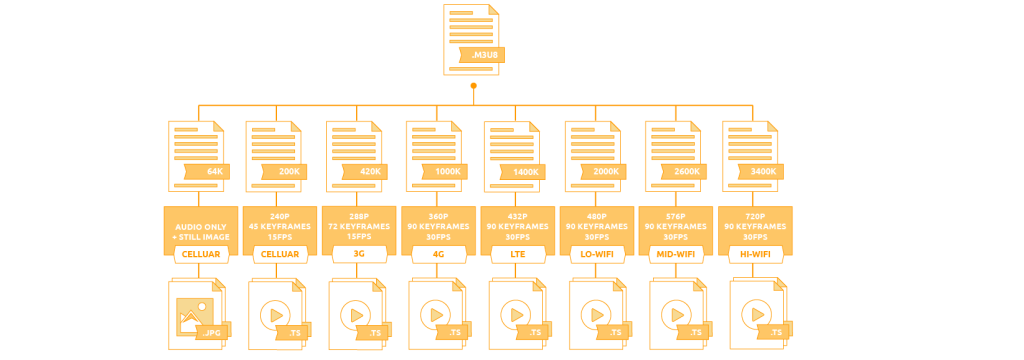
\includegraphics[scale=0.45]{figures/hls-segments.png} 
    \caption{Esquema de segmentação do protocolo HLS.}
    \small Fonte: https://www.encoding.com/http-live-streaming-hls/.
	\label{fig:hls_segments}
\end{figure}

A segmentação, retratada na figura \ref{fig:hls_segments}, compreende a divisão do vídeo em pequenos arquivos \text{TS} de mesma duração. Cada pedaço de mídia separado com sucesso é adicionado a um arquivo com extensão \textit{M3U8}, também chamado de \textit{playlist}. 

As \textit{playlists} são responsáveis por organizar os pedaços de forma sequencial para que o cliente consiga reproduzir a mídia corretamente. Cada \textit{playlist} contém URLs que indicam \textit{playlists} alternativas para diferentes qualidades de conexão. 

Fica então de responsabilidade do reprodutor HLS receber a \textit{playlist} do servidor, escolher a adequada banda larga disponível, agrupar os pedaços de vídeo e reproduzi-los em sequência. 

\section{Sistemas de suporte ao consumidor}

\subsection{Zendesk}

O Zendesk é uma plataforma paga que prove serviços de atendimento ao consumidor aos seus clientes. A plataforma tem o intuito de ajudar empresas a se relacionar melhor com os usuários, criando relações mais significativas\footnote{Disponível em: <https://www.zendesk.com/about>. Acesso em 20 mai. 2018.}. A principio o objetivo é fornecer suporte e melhorar o atendimento, para depois melhorar o relacionamento e o compromisso com o cliente.

\begin{figure}[ht!]
	\centering
		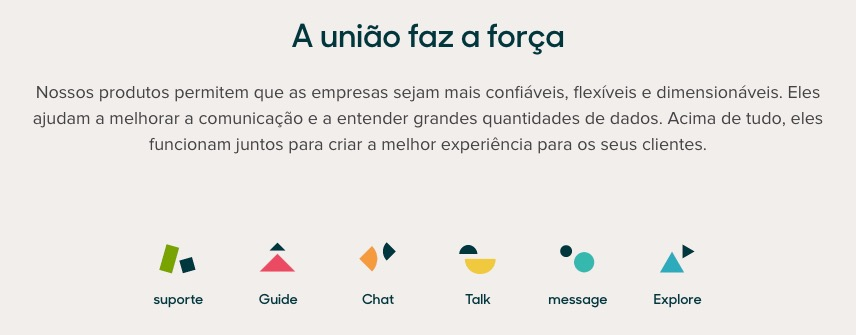
\includegraphics[scale=0.45]{figures/zendesk-modules.jpg} 
	\caption{Módulos disponíveis na plataforma}
	\label{fig:zendesk_modules}
\end{figure}

Composto por diversos módulos, ilustrados na \autoref{fig:zendesk_modules}, o software fornece assistência em diversas áreas: suporte ao cliente; capacitação de atendentes; troca de mensagens; ligações VoIP; e relatórios sobre os atendimentos.

\begin{figure}[ht!]
	\centering
		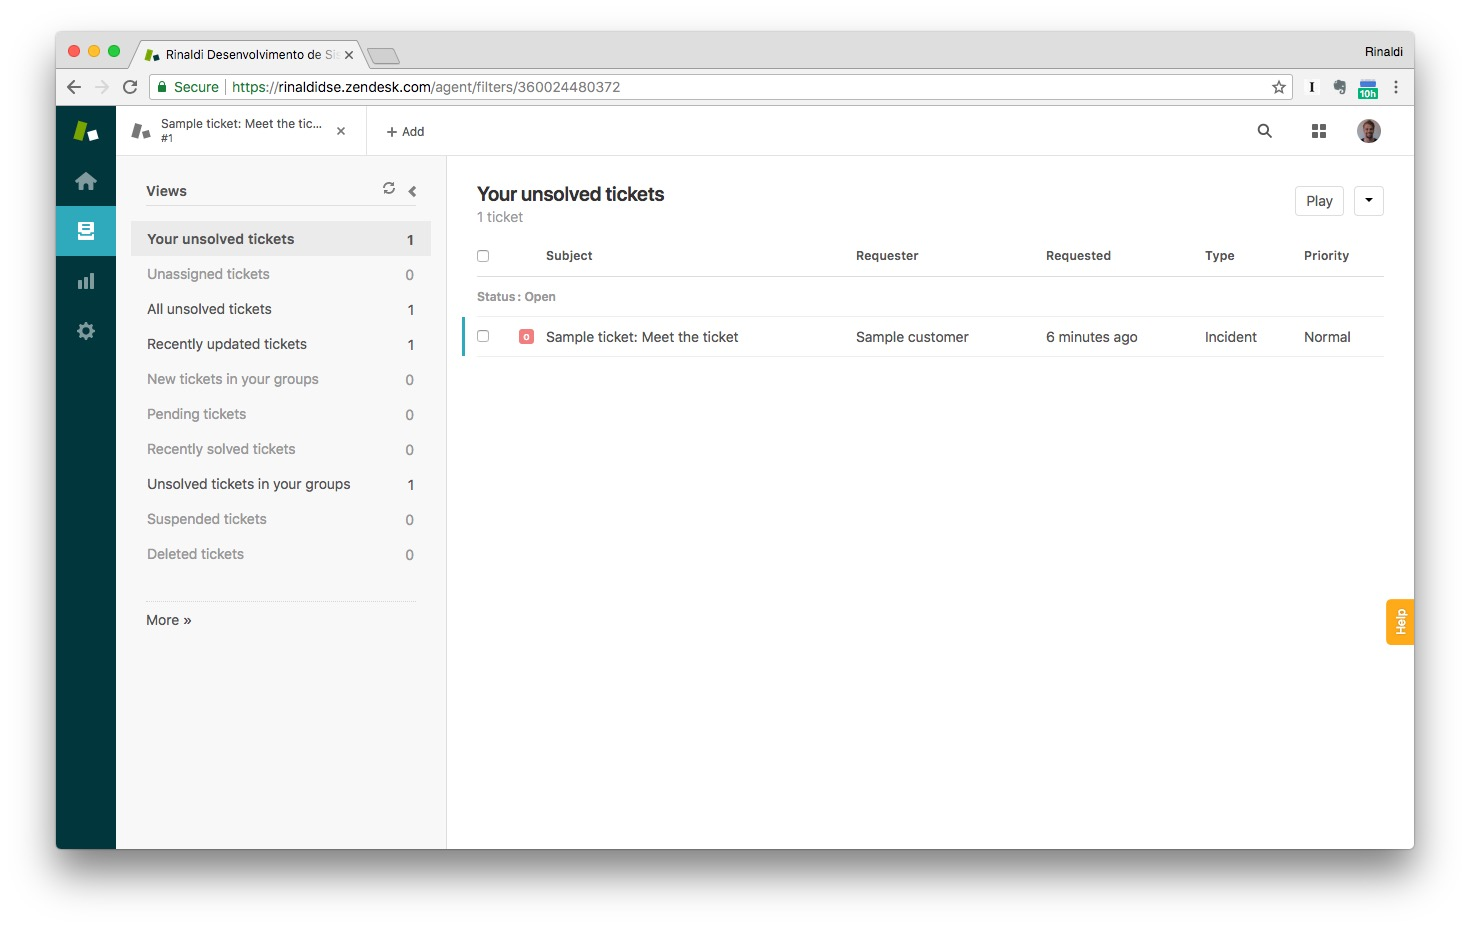
\includegraphics[scale=0.2]{figures/zendesk-ticket-overview.jpg} 
	\caption{Visão geral dos atendimentos}
	\label{fig:zendesk_ticket_overview}
\end{figure}

Atendimentos são chamados de \textit{tickets} dentro da plataforma. Esses contém informações do atendimento, e estão agrupados, sejam pendentes ou resolvidos, em uma só tela de visão geral, mostrada na \autoref{fig:zendesk_ticket_overview}.

\begin{figure}[ht!]
	\centering
		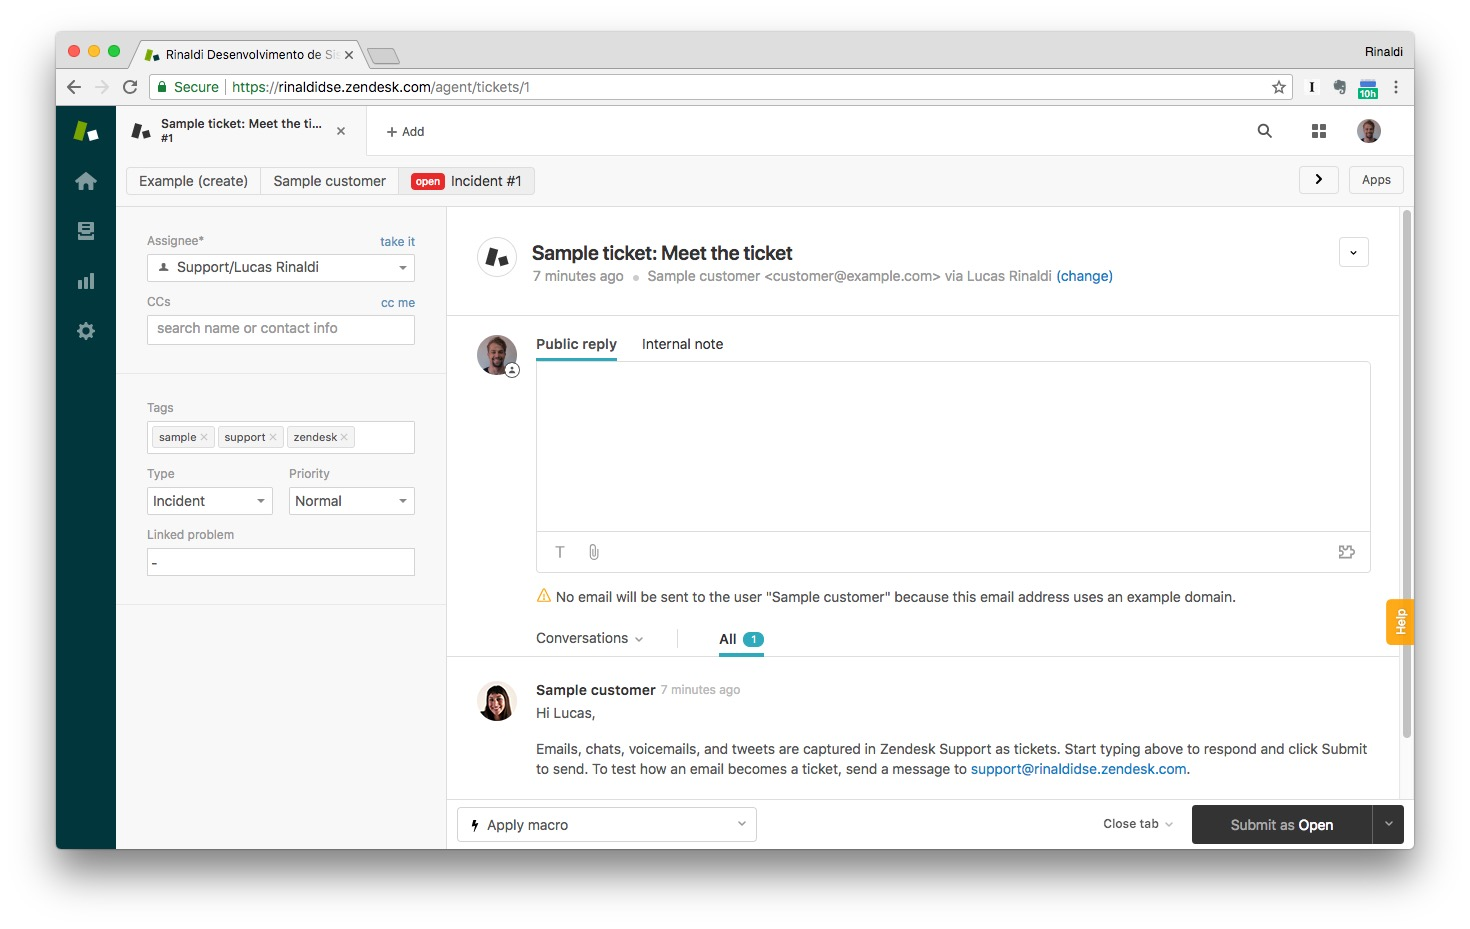
\includegraphics[scale=0.2]{figures/zendesk-ticket.jpg} 
	\caption{Visão interna do atendimento}
	\label{fig:zendesk_ticket}
\end{figure}

Cada \textit{ticket} possui suas próprias características, como prioridade, tipo e área correspondente da empresa (ver \autoref{fig:zendesk_ticket}). O contratante da plataforma pode escolher também por cadastrar um contrato SLA (\textit{Service Level Agreement}) de resolução de problemas, que fica à mostra para que os atendentes não estourem o limite.

Se o cliente necessita de atendimento em tempo real, a empresa pode utilizar um módulo de \textit{live chat}, por meio do qual o cliente entra em contato direto com um atendente designado pela empresa através de uma integração no site da mesma (ver \autoref{fig:zendesk_chat}).

\begin{figure}[ht!]
	\centering
		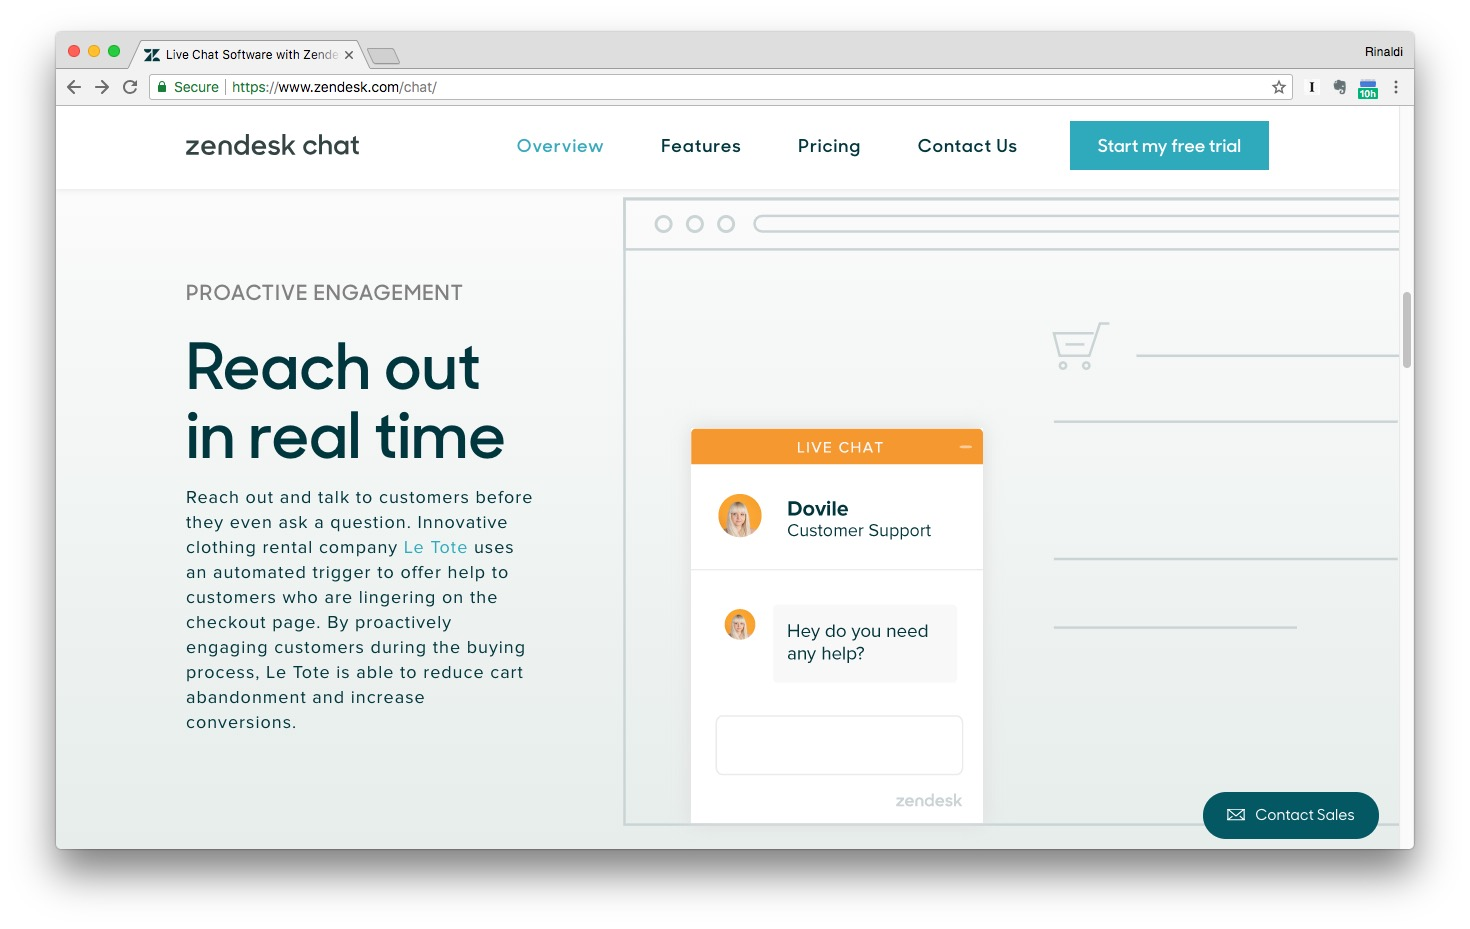
\includegraphics[scale=0.2]{figures/zendesk-chat.jpg} 
	\caption{Integração de chat no site do cliente}
	\label{fig:zendesk_chat}
\end{figure}

Apesar de esse atendimento acontecer somente por meio de troca de mensagens, outro módulo funciona com VoIP, porém não existem chamadas por vídeo.

Muito utilizado, Zendesk está presente em diversas \textit{startups} e grandes empresas, como AirBnB e OLX. Podemos ver mais exemplos na sua página de clientes\footnote{Disponível em: <https://www.zendesk.com/why-zendesk/customers>. Acesso em 20 mai. 2018.}.  A plataforma serviu de base para as primeiras ideias do projeto.
%FRANK: só é usado por startups? grandes empresas não usam?
%LUCAS: Adicionei e com referencias 

\subsection{Intercom}

Bastante voltada para soluções que colocam a troca de mensagens em foco\footnote{Disponível em: <https://www.intercom.com/about>. Acesso em 30 jun. 2017.}. Intercom possui múltiplos produtos que resolvem diferentes problemas nas empresas, todos com o objetivo de oferecer suporte e ajudar seus usuários diretos a reterem clientes.

O modelo de múltiplos produtos dá ao cliente oportunidade de escolher cada um separadamente. São eles \textit{Messenger}, \textit{Inbox} e \textit{Articles}.

%FRANK: essa figura não traz nenhuma informação técnica sobre o produto, não me parece apropriada para um TCC, serve só para marketing
\begin{figure}[ht!]
	\centering
		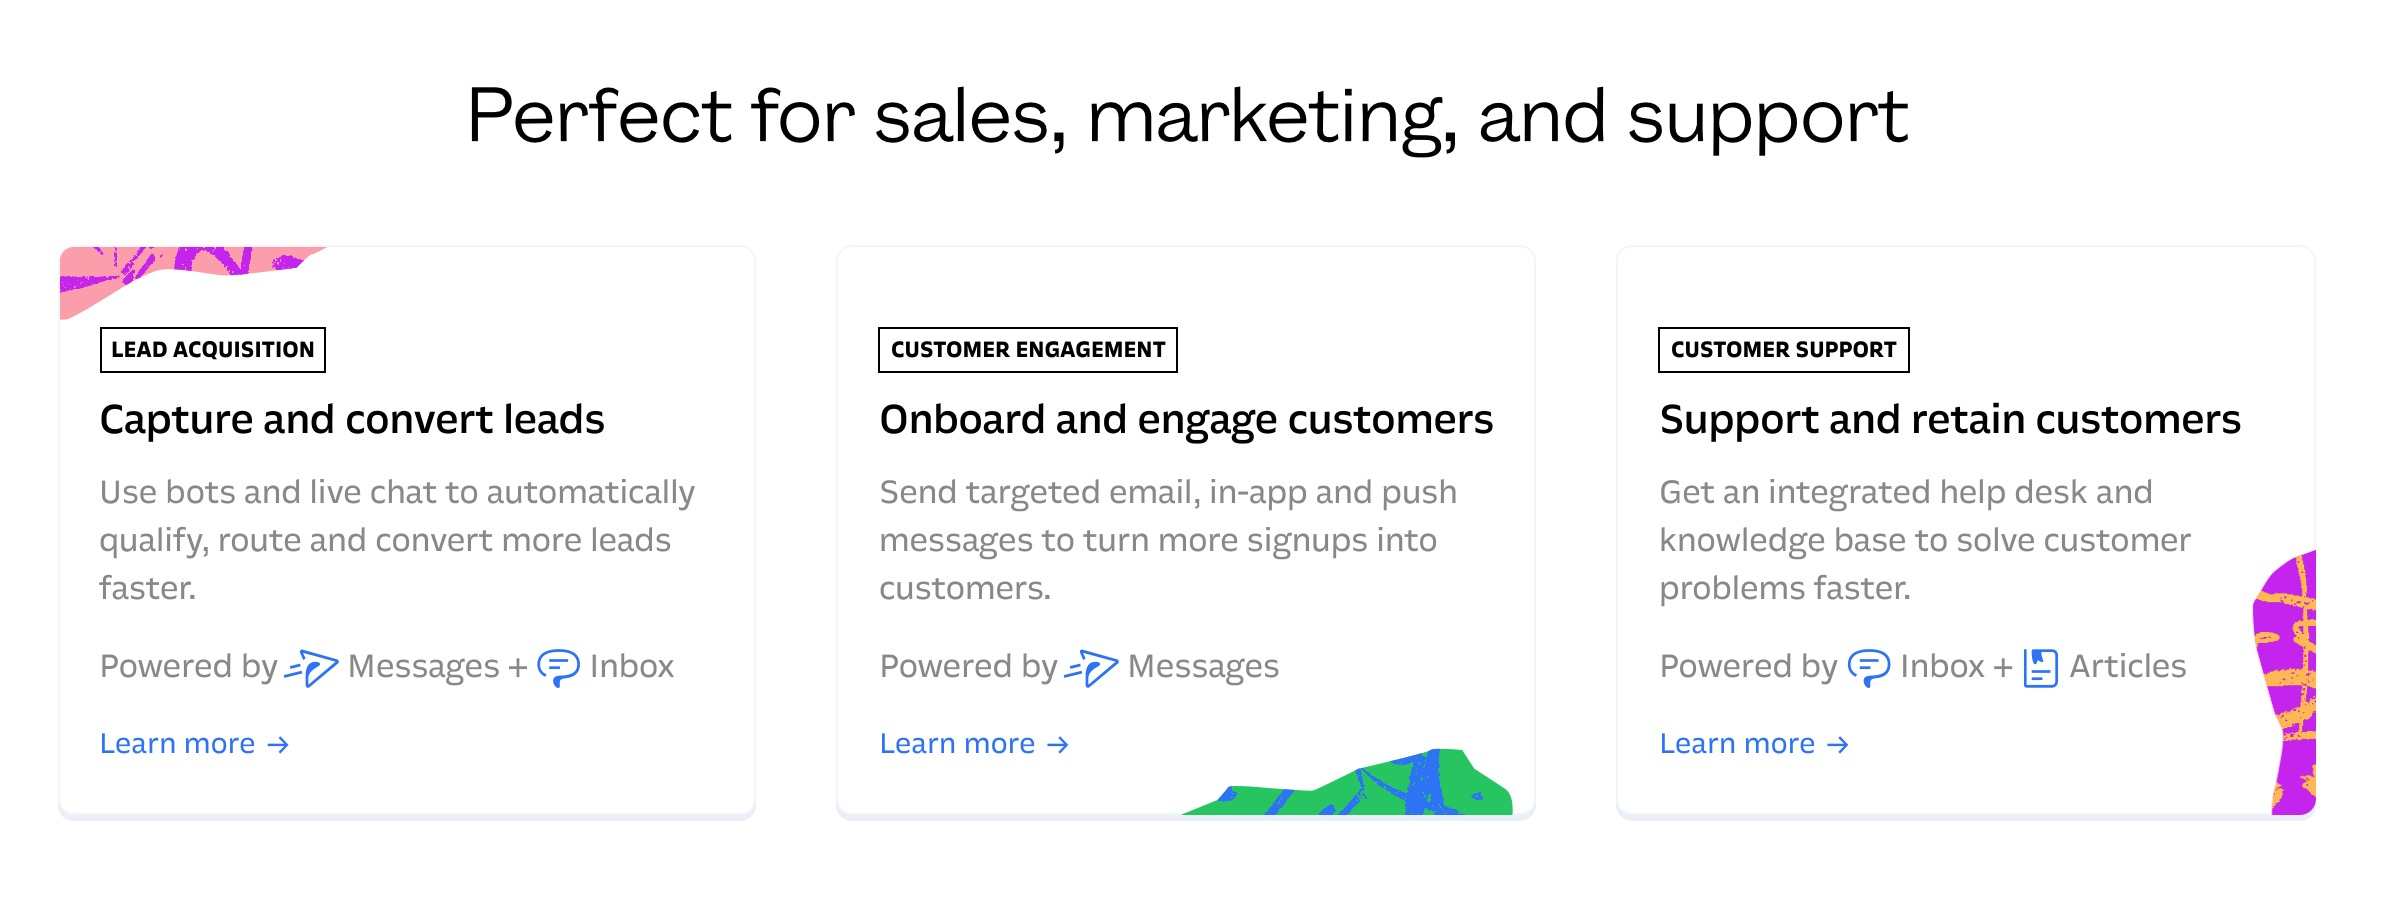
\includegraphics[scale=0.2]{figures/intercom-use-cases.jpg} 
	\caption{Produtos e casos de uso do Intercom}
	\label{fig:intercom_use_cases}
\end{figure}

Além da liberdade, podemos ver em \autoref{fig:intercom_use_cases} as sugestões de combinações dentro da plataforma para cada especifico caso de uso de acordo com a sua necessidade.

Nota-se que diferentemente do Zendesk, a empresa direciona grande parte de seus esforços a área de retenção de clientes. Coloca-os em etapas de funil de vendas e utilizando o seu produto \textit{Messenger} envia mensagens de acordo com a etapa atual. No projeto apresentado nesse trabalho não temos um foco em marketing ou vendas, por isso a pequena explicação.

Como citado acima, seus produtos prezam pela troca de mensagens. O módulo \textit{Inbox} funciona como um \text{live chat} integrado no site do usuário, conectando assim o seu cliente com atendentes de suporte.

\begin{figure}[ht!]
	\centering
		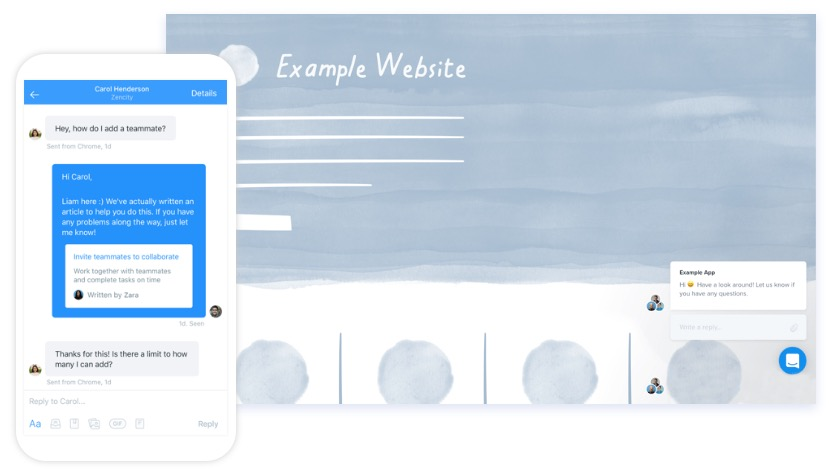
\includegraphics[scale=0.4]{figures/intercom-inbox.jpg} 
	\caption{Intercom Inbox}
	\label{fig:intercom_inbox}
\end{figure}

Sua vantagem é possuir um conexão facilitada com \textit{Articles}, seu outro produto, e assim fazer com que o atendente resolva os problemas de forma rápida e fácil.

\textit{Articles} é uma central de ajuda, onde guias sobre o \textit{software} e perguntas mais frequentes podem ser publicadas para melhor resolução de problemas. 

\begin{figure}[ht!]
	\centering 
		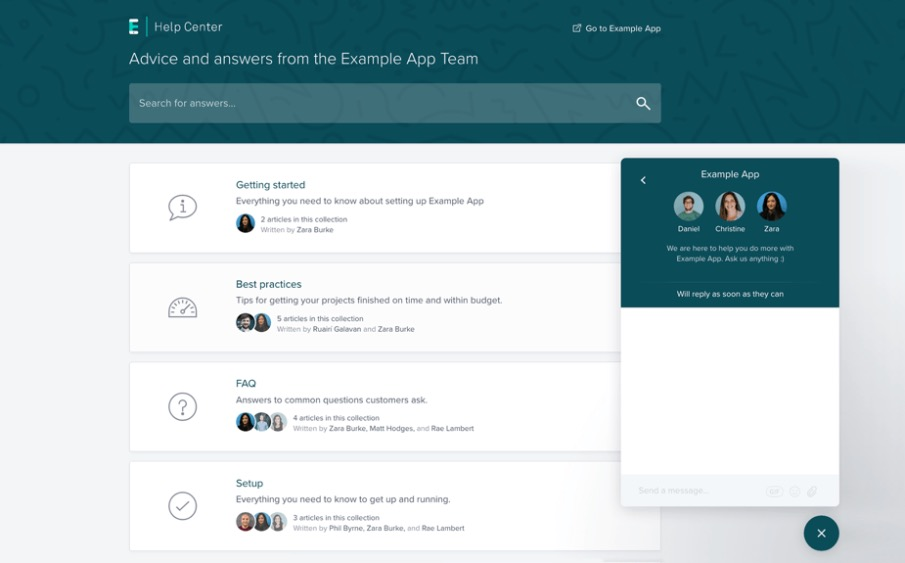
\includegraphics[scale=0.4]{figures/intercom-articles.jpg} 
	\caption{Intercom Articles}
	\label{fig:intercom_articles}
\end{figure}

A integração com o \textit{Inbox} serve para que o seu time consiga escalar o suporte. No momento que o atendente recebe uma palavra-chave a central de ajuda retorna uma lista de artigos relacionados à mesma. 

Traz também relatórios e ações sobre como os clientes estão utilizando a central e como melhora-lá. Na \autoref{fig:intercom_articles_actions} vemos exemplos de ações a serem tomadas.

\begin{figure}[ht!]
	\centering 
		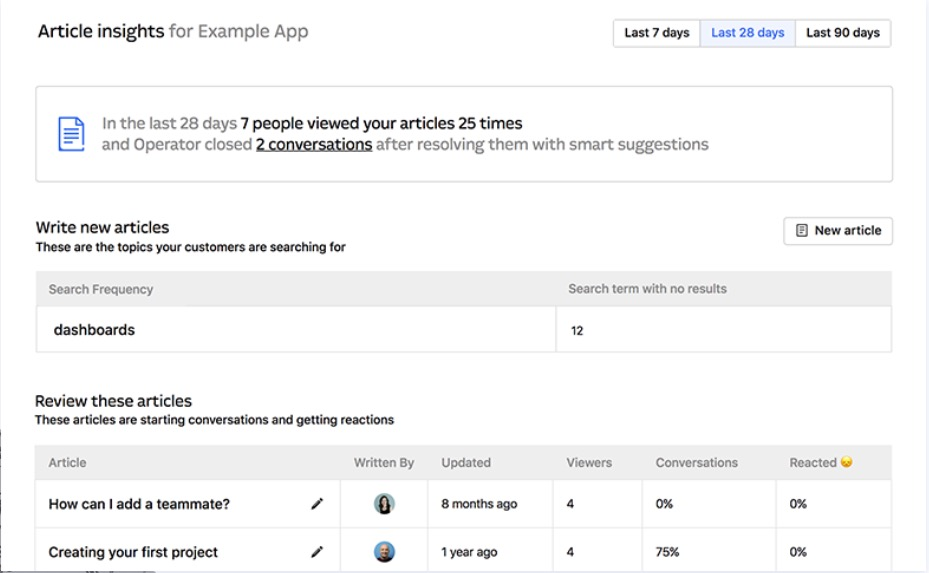
\includegraphics[scale=0.4]{figures/intercom-articles-actions.jpg} 
	\caption{Relatório e ações no Intercom Articles}
	\label{fig:intercom_articles_actions}
\end{figure}

Centrado e com produtos voltados para o marketing algumas funcionalidades divergem do objetivo desse projeto, porém o Intercom serviu de inspiração para ideias futuras. 

A integração da central de ajuda dentro do chat é um recurso poderoso que poderia ser integrado dentro de uma videoconferência. Em tempo real o atendente pode pesquisar sobre o assunto que o cliente está falando e indicar a resposta certa, facilitando a resolução do problema.

